% =====================================================================
% Argos — Product Requirements Document (PRD)
% A Multi-Agent LLM Trading Research Desk
% IEEE conference format (IEEEtran), Overleaf-ready
%
% Compile: pdflatex → bibtex → pdflatex × 2
% =====================================================================
\documentclass[conference]{IEEEtran}

\usepackage{cite}          % [1]-[3] style citation compression
\usepackage{amsmath,amssymb,amsfonts}
\usepackage{graphicx}
\usepackage{booktabs}      % professional tables
\usepackage{array}
\usepackage{tabularx}
\usepackage{enumitem}
\usepackage{url}
\usepackage{tikz}
\usetikzlibrary{arrows.meta,positioning,shapes.geometric}
\usepackage[colorlinks=true,linkcolor=black,citecolor=black,urlcolor=black]{hyperref}

% ---- Shorthand ------------------------------------------------------
\newcommand{\sys}{Argos}
\newcolumntype{L}[1]{>{\raggedright\arraybackslash}p{#1}}

\begin{document}

\title{\sys{}: A Multi-Agent Large Language Model Trading Research Desk\\
\large Product Requirements Document and Research Plan (v1.0)}

\author{\IEEEauthorblockN{Kishor Timilsena}
\IEEEauthorblockA{\textit{Fusemachines AI Fellowship 2026}\\
% TODO: replace with your institution / affiliation
Kathmandu, Nepal\\
kishor.timilsena@example.com}}

\maketitle

% =====================================================================
\begin{abstract}
Large language models (LLMs) can pull useful trading signals out of news and company data, and recent systems organize several LLMs into a team with different roles. But in most published systems the LLMs do the whole job: the same model reads the news, decides what it means, argues about it, and sizes the trade. This document specifies \sys{}, a multi-agent \emph{research desk} that produces one trading recommendation per ticker per day---BUY, SELL, or HOLD, with a confidence score, a position cap, and a complete written trail of how the decision was made. A human trader reads this before acting; the system never places orders. Three design choices set \sys{} apart from earlier work. First, \textbf{two kinds of intelligence, not one}: five LLM roles work alongside Kronos, a foundation model trained on candlestick data, and the desk uses Kronos's full forecast distribution---not just its average forecast. Second, \textbf{a forced argument}: a Bull agent and a Bear agent must respond to each other's actual claims before anything is decided. Third, \textbf{belief is not permission}: the debate only says what the desk believes; a separate Risk Manager decides what the desk is allowed to do. The Risk Manager reads the debate and the width of Kronos's forecast bands, caps the position size, and can veto the trade outright---sending the pipeline straight to HOLD. We specify the product requirements, the graph architecture, each agent's inputs and outputs, how models are assigned under free-tier API limits, a walk-forward evaluation with three baselines and four ablations, and a stress test for the veto. Every research claim is stated so that a specific test can prove it wrong. The deliverable is a decision with a full, checkable explanation---not profit.
\end{abstract}

\begin{IEEEkeywords}
multi-agent systems, large language models, decision support, algorithmic trading, foundation models, time-series forecasting, risk management, adversarial debate, evaluation methodology
\end{IEEEkeywords}

% =====================================================================
\section{Introduction}
% =====================================================================

\subsection{Motivation}

Before placing a trade, a trader usually checks a few things: what the company's numbers say, what the news says, what the chart says, an argument between the bull case and the bear case, and finally a risk check that can say no. What makes a research desk good is not any single analyst---it is how the roles interact: who sees what, who can overrule whom, and which evidence survives the argument. Recent work shows that LLMs can play these roles: ChatGPT-style models predict stock moves from headlines better than classic sentiment scores \cite{lopezlira2023chatgpt}, and TradingAgents \cite{xiao2024tradingagents} shows that a team of role-specialized LLM agents---analysts, bull and bear researchers, a risk team, and a trader---can run a pipeline that mirrors a real trading firm.

Two gaps motivate this project.

\subsubsection{One model plays every role} In most LLM trading agents \cite{xiao2024tradingagents,yu2023finmem}, every ``analyst'' is the same underlying model reading different text. The number-crunching leg---the actual price forecast---is either missing or reduced to chart indicators (RSI, MACD) that the LLM then re-explains in words. This mixes two different skills: finding patterns in numbers, and combining messy evidence into a judgment. A time-series model is built for the first; an LLM is built for the second. Kronos \cite{shi2025kronos}, a foundation model trained on candlestick data from over 45 exchanges, is a strong open-source option for the first. \sys{} makes it a full member of the desk with one strict rule: its forecast is narrated as-is, never re-interpreted (Section~\ref{sec:arch-kronos}).

\subsubsection{Nobody can say no} In published systems, the step that decides direction also decides size. No independent agent can reject the trade. \sys{} splits the two questions: the debate answers \emph{what do we believe?}, and the Risk Manager answers \emph{what are we allowed to do?} The Risk Manager reads the debate and the width of Kronos's forecast bands---how spread out its sampled forecasts are. A confident-sounding debate cannot override a wide band. As far as we know, this kind of risk layer---one that reads forecast uncertainty and can block or shrink a trade no matter what the debate says---is the main new contribution of this project (Section~\ref{sec:related-pos}).

Finally, the product is deliberately limited: \sys{} advises, and it never trades. The output is a recommendation with a full trail that a human reviews before acting. No orders, no real money. This one constraint shapes the whole evaluation plan (Section~\ref{sec:eval}): we audit the reasoning, not the profit.

\subsection{Project Context and Constraints}

\sys{} is a solo fellowship project. It runs under hard constraints that shape the design:

\begin{itemize}[leftmargin=*,itemsep=1pt,topsep=2pt]
  \item \textbf{Free tiers only:} two Google Cloud projects give two separate Gemini quota pools; Kronos runs as a batch job on free GPU sessions. Nothing costs money.
  \item \textbf{One person, about 3 hours a day:} this favors simple, debuggable code over clever architecture.
  \item \textbf{Fixed scope:} 1--3 tickers, one walk-forward backtest window, one stress-test window. Scaling to more tickers or more market regimes is future work.
  \item \textbf{The unit of value is a defensible decision trail,} logged as structured JSON for every run.
\end{itemize}

\subsection{What This Document Contributes}

This document is both a PRD and a research plan. It contributes:

\begin{enumerate}[leftmargin=*,itemsep=1pt,topsep=2pt]
  \item \textbf{A full PRD:} who uses the desk, what it must do, prioritized requirements with acceptance targets, and product KPIs (Section~\ref{sec:product}).
  \item \textbf{A detailed architecture:} a stateful LangGraph pipeline with parallel analysts, a two-side debate in sequence, veto-based branching, a typed output schema per agent, one central model table, and a no-lookahead data rule enforced in one place (Section~\ref{sec:arch}).
  \item \textbf{A way of combining an LLM desk with a candlestick foundation model,} where the forecast's spread---not its point value---drives both the technical view and the risk sizing (Section~\ref{sec:arch-kronos}).
  \item \textbf{A falsifiable evaluation plan:} a walk-forward protocol, three baselines, four ablations, metrics in four families, and a stress test for the veto (Section~\ref{sec:eval}).
  \item \textbf{Six research hypotheses} with explicit measurement and falsification criteria (Section~\ref{sec:hypotheses}).
\end{enumerate}

% =====================================================================
\section{Background and Related Work}
\label{sec:related}
% =====================================================================

\subsection{LLM Agents in Trading}
After chat-style LLMs became widely available, trading agents followed fast. FinMem \cite{yu2023finmem} gives a single LLM agent layered memory and a fixed character, then lets it trade. FinGPT \cite{yang2023fingpt} and BloombergGPT \cite{wu2023bloomberggpt} provide open and proprietary financial LLMs. MarketSenseAI \cite{fatouros2024marketsenseai} wraps LLMs into a queryable stock-prediction service. Lopez-Lira and Tang \cite{lopezlira2023chatgpt} give the clearest evidence that LLMs extract return-predictive signal from news text. Ding et al.\ \cite{ding2024llmtrading} survey the field and find that most systems share the same shape---analysts feed a decision step---with little real debate and no independent risk gate. TradingAgents \cite{xiao2024tradingagents} is the closest system: fundamental, sentiment, technical, and news analysts; bull and bear researchers; a risk team; and a trader agent. \sys{} borrows the desk idea but differs in three ways: the technical leg is a dedicated candlestick foundation model instead of an LLM re-reading indicators; the risk layer holds a real veto instead of advisory influence; and the product is decision support with auditable trails, not autonomous trading.

\subsection{Multi-Agent Debate}
When LLMs critique each other's answers over several rounds, their factuality and reasoning improve \cite{du2023debate}. Role-prompted debate also pushes models to consider more possibilities than a single agent answering alone \cite{liang2023divergent}. ChatEval \cite{chan2023chateval} shows debate-style judging improves evaluation, and Smit et al.\ \cite{smit2024mad} compare debate strategies and find that the choice of format matters---with two warnings: debate costs extra calls, and agents can converge too early. Surveys of LLM multi-agent systems \cite{guo2024llmmultiagents} name communication structure and role assignment as first-order design choices. \sys{} uses the smallest useful version: a two-turn debate in which the Bear must rebut the Bull's specific claims. This fits the free-tier budget; more rounds are a settings change, not a redesign. The classic failure of groups---groupthink \cite{janis1972groupthink}---is treated as a measurable bug: if the Bull and Bear always report similar confidence, the debate is decoration. H4 tests exactly this (Section~\ref{sec:hypotheses}).

\subsection{Time-Series Foundation Models}
Transformers underpin modern forecasting \cite{vaswani2017attention,nie2023patchtst}, and pretrained language models transfer well to time series \cite{zhou2023onefitsall}. Foundation models for probabilistic forecasting---Lag-Llama \cite{rasul2023lagllama} and Chronos \cite{ansari2024chronos}---established the idea of pretraining on tokenized time series. Kronos \cite{shi2025kronos} is the first open-source foundation model built for financial candles: a tokenizer turns OHLCV bars into discrete tokens, and a decoder-only Transformer generates future bars one by one. Because it samples, it naturally produces a \emph{distribution} of forecast paths, not one line. We use exactly that: the p90--p10 spread of the sampled paths (the ``uncertainty width'') becomes the Risk Manager's main numeric input. Forecast quality is scored with MASE \cite{hyndman2006another} and WQL, separately from trading outcomes, following Kronos's own evaluation.

\subsection{Market Context}
The Efficient Markets Hypothesis \cite{fama1970efficient} is the skeptical baseline: after costs, rules based on public information should not systematically make money. The Adaptive Markets Hypothesis \cite{lo2004adaptive} explains when inefficiencies may appear and disappear---which frames \sys{} as a daily research desk, not a claimed trading strategy. Prospect theory \cite{kahneman1979prospect} and the heuristics-and-biases literature \cite{tversky1974judgment} document overconfidence and loss aversion in human judgment; an explicit Bear Advocate and a veto-wielding Risk Manager are structural answers to those biases. The Sharpe ratio \cite{sharpe1994sharpe} and maximum drawdown remain our risk measures (simulated; nothing is executed).

\subsection{Positioning}
\label{sec:related-pos}
Table~\ref{tab:positioning} sums up the gap. The claim is deliberately narrow and testable: \textbf{a veto-first risk layer that reads forecast uncertainty and can override the debate}, inside a decision-support product.

\begin{table}[!t]
\centering
\caption{Positioning against representative systems.}
\label{tab:positioning}
\small
\begin{tabularx}{\columnwidth}{L{1.55cm} X X X}
\toprule
& \textbf{TradingAgents} \cite{xiao2024tradingagents} & \textbf{FinMem} \cite{yu2023finmem} & \textbf{\sys{} (this work)} \\
\midrule
Technical signal & LLM reads indicators & LLM reads price/news stream & Kronos candlestick foundation model \cite{shi2025kronos} \\
\addlinespace[2pt]
Debate & Bull/Bear researcher debate & Single agent, no debate & Two-turn debate; Bear must rebut Bull's actual claims \\
\addlinespace[2pt]
Risk layer & Risk team (advises the trader) & Risk appetite set by the character prompt & Veto power; reads forecast uncertainty; size cap enforced in code \\
\addlinespace[2pt]
Product & Trading decisions & Trading decisions & Decision support; full audit trail; no execution \\
\addlinespace[2pt]
Evaluation & Cumulative returns & Return metrics vs.\ baselines & Decision quality + forecast quality + veto behavior + auditability \\
\bottomrule
\end{tabularx}
\end{table}

% =====================================================================
\section{Problem, Scope, and Non-Goals}
\label{sec:problem}
% =====================================================================

\subsection{What the System Must Produce}

The system looks at one ticker from a fixed universe of 1--3 tickers on one date $t$. It may use only information known by that date: price history, filings, news. It outputs:

\begin{equation}
D_t(s) = \big(a,\; c,\; w,\; \mathcal{R}_t\big)
\label{eq:decision}
\end{equation}

where $a \in \{\textsc{buy}, \textsc{sell}, \textsc{hold}\}$ is the recommended action, $c \in [0,1]$ is a confidence score, $w \in [0,1]$ is the largest position the Risk Manager allows, and $\mathcal{R}_t$ is the full reasoning trail---every agent's output, saved as written. A human trader reads all of this before doing anything. The system never sends orders; $w$ only sizes a hypothetical position for research scoring.

\subsection{Who Uses It, and How}

\begin{table}[!t]
\centering
\caption{Users and what they do with the desk.}
\label{tab:users}
\small
\begin{tabularx}{\columnwidth}{L{1.5cm} X}
\toprule
\textbf{User} & \textbf{Main use} \\
\midrule
Trader (human) & Reads the daily desk brief---the decision, the confidence, the bull/bear summary, and the risk cap---before placing an order. Opens the full reasoning trail when the recommendation disagrees with their own view. \\
\addlinespace[2pt]
Researcher (the solo maintainer) & Re-runs the pipeline on cached data while fixing one agent; reads debate transcripts to check the argument is real; runs the ablations. \\
\addlinespace[2pt]
Reviewer / evaluator & Checks that trails are complete, outputs match the schemas, and no future data leaked in; reproduces a decision from cached inputs; checks the veto during the stress window. \\
\bottomrule
\end{tabularx}
\end{table}

\subsection{Non-Goals (Explicit)}

\begin{itemize}[leftmargin=*,itemsep=1pt,topsep=2pt]
  \item No order execution, no broker connection, no paper-trading fills in this phase (that is a stretch goal only).
  \item No portfolio building across many tickers; no multiple timeframes or strategies.
  \item No always-on live infrastructure; Kronos runs in batch and its forecasts are cached.
  \item No claim of profit. The deliverable is an honest, auditable decision process with real baselines---including results where the system loses.
\end{itemize}

\subsection{Assumptions and Constraints}

Free Gemini tiers across two cloud projects; yfinance for prices; free news and filings sources; Kronos-small/base on CPU or a free Colab GPU with a 512-candle context; Python 3.11+; LangGraph for orchestration; Pydantic v2 for output schemas; pytest with fixture data (no live API calls in unit tests).

% =====================================================================
\section{Product Requirements}
\label{sec:product}
% =====================================================================

\subsection{Functional Requirements}

\begin{table}[!t]
\centering
\caption{Functional requirements (P1 = must ship; P2 = should ship; P3 = later).}
\label{tab:fr}
\small
\begin{tabularx}{\columnwidth}{L{0.75cm} X L{0.85cm}}
\toprule
\textbf{ID} & \textbf{Requirement} & \textbf{Priority} \\
\midrule
FR-1 & Produce a decision per ticker and date per Eq.~\ref{eq:decision}: action, confidence, position cap, full rationale. & P1 \\
FR-2 & Every agent output must be a schema-validated structured object (Pydantic); no parsing of free text. & P1 \\
FR-3 & The three analysts run in parallel; the debate runs in order (Bull, then Bear); the Bear must address the Bull's specific claims. & P1 \\
FR-4 & The Risk Manager returns one of three verdicts: approve, shrink the cap, or veto. A veto short-circuits the graph to HOLD in plain code, with no extra LLM call. & P1 \\
FR-5 & The final position size never exceeds the Risk Manager's cap; enforced in code, not in the prompt. & P1 \\
FR-6 & No-lookahead guard: one data loader is the only code that reads raw data, and it fails hard if any data is newer than the evaluation date. & P1 \\
FR-7 & Every run logs a full reasoning trail (JSONL): all agent outputs, verdicts, errors, and run metadata. & P1 \\
FR-8 & The Technicals agent narrates Kronos's forecast as-is; making up causes is forbidden by its prompt. & P1 \\
FR-9 & Model routing lives in one central table: agent $\rightarrow$ (API key, model). Rebalancing requires no changes to agent code. & P1 \\
FR-10 & Debate depth (rounds $N \ge 1$) is configurable; default 1 round. & P2 \\
FR-11 & Multi-round debate with a judge-style synthesis (cf.\ \cite{smit2024mad}). & P3 \\
FR-12 & Paper-trading hookup (Alpaca sandbox) as a forward-looking test harness. & P3 \\
\bottomrule
\end{tabularx}
\end{table}

\subsection{Non-Functional Requirements}

\begin{table}[!t]
\centering
\caption{Non-functional requirements.}
\label{tab:nfr}
\small
\begin{tabularx}{\columnwidth}{L{0.85cm} X L{1.6cm}}
\toprule
\textbf{ID} & \textbf{Requirement} & \textbf{Target} \\
\midrule
NFR-1 & Share of agent outputs that pass schema validation & 100\% (invalid $\Rightarrow$ logged error, run continues) \\
NFR-2 & Share of decisions where every upstream field is present or explicitly marked failed & 100\% \\
NFR-3 & Data-leakage incidents across the full backtest & 0 (enforced in code and spot-audited) \\
NFR-4 & Cost per decision & \$0 (free tier) \\
NFR-5 & Time to produce one decision (7 LLM calls + cached forecast) & $\le$ 3 minutes \\
NFR-6 & Any logged decision can be rebuilt from cached inputs and config & every run \\
NFR-7 & Unit tests run without network access & all node tests \\
\bottomrule
\end{tabularx}
\end{table}

\subsection{Product KPIs}

Because the product is a research desk, we measure the quality of its reasoning, not money: (i) \textbf{coverage}---the share of trading days with a well-formed decision; (ii) \textbf{audit coverage}---the share of decisions with a complete trail (target 100\%); (iii) \textbf{veto calibration}---the veto must fire more often in the stress window than in calm periods; (iv) \textbf{usefulness}---a human reads sample daily briefs and rates them (Section~\ref{sec:eval-human}).

% =====================================================================
\section{System Architecture}
\label{sec:arch}
% =====================================================================

\subsection{Overview}

\sys{} runs once per ticker per day. Seven agent roles work through one shared state object. No agent calls another agent directly---they only read and write shared state. Figure~\ref{fig:arch} shows the wiring.

\begin{figure}[!t]
\centering
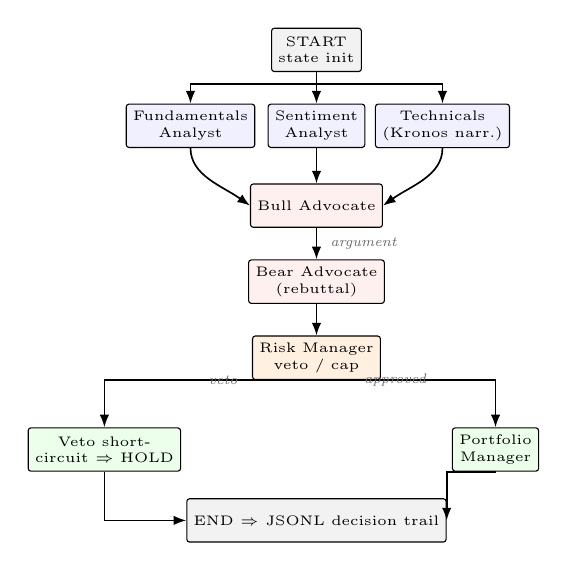
\begin{tikzpicture}[
  node distance=4mm and 5mm,
  box/.style={draw, rounded corners=1pt, align=center, inner sep=2.5pt, font=\tiny, minimum height=5.5mm},
  analyst/.style={box, fill=blue!6},
  debate/.style={box, fill=red!6},
  risk/.style={box, fill=orange!12},
  pm/.style={box, fill=green!8},
  io/.style={box, fill=gray!10},
  lbl/.style={font=\tiny\itshape, text=black!60},
  line/.style={-{Latex[length=1.6mm]}, semithick}
]
\node[io] (start) {START\\state init};
\node[analyst, below=of start, xshift=-16mm] (fund) {Fundamentals\\Analyst};
\node[analyst, below=of start] (sent) {Sentiment\\Analyst};
\node[analyst, below=of start, xshift=16mm] (tech) {Technicals\\(Kronos narr.)};
\node[debate, below=4.5mm of sent] (bull) {Bull Advocate};
\node[debate, below=of bull] (bear) {Bear Advocate\\(rebuttal)};
\node[risk, below=of bear] (risk) {Risk Manager\\veto / cap};
\node[pm, below left=6mm and 9mm of risk] (hold) {Veto short-\\circuit $\Rightarrow$ HOLD};
\node[pm, below right=6mm and 9mm of risk] (pm) {Portfolio\\Manager};
\node[io, below=15mm of risk] (endn) {END $\Rightarrow$ JSONL decision trail};

\draw[line] (start.south) -- ++(0,-1.5mm) -| (fund.north);
\draw[line] (start.south) -- (sent.north);
\draw[line] (start.south) -- ++(0,-1.5mm) -| (tech.north);
\draw[line] (fund.south) .. controls +(0,-0.35) and +(-0.35,0.25) .. (bull.west);
\draw[line] (sent.south) -- (bull.north);
\draw[line] (tech.south) .. controls +(0,-0.35) and +(0.35,0.25) .. (bull.east);
\draw[line] (bull.south) -- node[lbl, right=0.5mm] {argument} (bear.north);
\draw[line] (bear.south) -- (risk.north);
\draw[line] (risk.south) -| node[lbl, pos=0.22] {veto} (hold.north);
\draw[line] (risk.south) -| node[lbl, pos=0.22] {approved} (pm.north);
\draw[line] (hold.south) |- (endn.west);
\draw[line] (pm.south) -| (endn.east);
\end{tikzpicture}
\caption{The \sys{} graph. Blue: the three analysts run in parallel (one of them narrates Kronos). Red: the Bull and Bear argue in sequence. Orange: the Risk Manager can veto. Green: final synthesis, or a straight-to-HOLD shortcut on veto.}
\label{fig:arch}
\end{figure}

\subsection{How the Agents Are Wired (LangGraph)}

We use LangGraph \cite{langgraph2024} to run the pipeline. We chose it over CrewAI and AutoGen because the problem is a fixed workflow with parallel steps and conditional branches---not a free conversation between agents. Three decisions matter most:

\subsubsection{One shared state object} A single \texttt{TypedDict} (\texttt{FuseState}) flows through every node. Nodes add their own fields and never change what earlier agents wrote. This makes the audit trail almost free: every intermediate output already sits in one place, ready to log. The error list is append-only (an \texttt{operator.add} reducer), so the parallel analysts can report failures at the same time without overwriting each other.

\subsubsection{Two failure rules} Agents fail soft: if an analyst crashes, the error is logged into state, its signal is set to \texttt{None}, and the run continues; downstream agents see an explicit ``(no output --- agent may have failed)'' note instead of a silent gap. The data loader fails fast: any data-integrity problem stops the run immediately (Section~\ref{sec:arch-data}).

\subsubsection{Parallel fan-out, implicit join} The entry node sends work to all three analysts at once, and LangGraph runs them concurrently. The join needs no extra code: the Bull node simply takes input from all three, and the framework waits for all of them.

\subsection{Agent Roles and Their Contracts}

Each agent has three things: its own prompt file (no shared mega-prompt), a Pydantic schema bound to the LLM call with \texttt{.with\_structured\_output()}, and a fixed slot in the shared state. The contracts are the core of the design: agents exchange typed data, not free text.

\begin{table}[!t]
\centering
\caption{Agent roster: inputs, outputs, contracts.}
\label{tab:roster}
\small
\begin{tabularx}{\columnwidth}{L{1.35cm} L{1.7cm} L{1.55cm} X}
\toprule
\textbf{Agent} & \textbf{Input} & \textbf{Output schema} & \textbf{Contract} \\
\midrule
Fundamentals & Filing excerpts, earnings-call transcript, pre-computed ratios & \texttt{AnalystSignal} & Every number in the rationale must come from the provided inputs; $\le$150 words. \\
\addlinespace[2pt]
Sentiment & Headlines (5--10 days), rating changes, social volume if available & \texttt{AnalystSignal} & Weighs recency and source quality; if data is thin, returns neutral with low confidence. \\
\addlinespace[2pt]
Technicals & Kronos forecast distribution & \texttt{AnalystSignal} & \emph{Narration only}: describe the forecast, the spread, and the width; no invented causes. \\
\addlinespace[2pt]
Bull Advocate & All three analyst outputs & \texttt{DebateArgument} & Strongest buy case; must face conflicting signals head-on; names its single strongest piece of evidence. \\
\addlinespace[2pt]
Bear Advocate & Analyst outputs + \emph{Bull's full argument} & \texttt{DebateArgument} & Must rebut the Bull's specific claims (quoted), not give a generic bear case. \\
\addlinespace[2pt]
Risk Manager & Debate outputs, Kronos uncertainty width, (portfolio state) & \texttt{RiskVerdict} & \texttt{veto} flag + \texttt{max\_position\_size} cap; wide uncertainty $\Rightarrow$ tighter cap, no matter how confident the debate sounded. \\
\addlinespace[2pt]
Portfolio Manager & Complete trail + risk verdict & \texttt{FinalDecision} & Final action; size $\le$ risk cap (enforced in code); disagreements recorded in \texttt{dissent\_notes}. \\
\bottomrule
\end{tabularx}
\end{table}

All four schemas share a shape: a stance (bullish/bearish/neutral, or buy/sell/hold), a numeric confidence between 0 and 1 (numbers, not ``high/medium/low''---we need numbers for the calibration tests), a short list of key factors (at most 5, or 3 for risk), and a reasoning field with a word limit. The debate schemas add \texttt{strongest\_evidence} and \texttt{rebuttal\_of\_opposing\_view}. The final schema adds \texttt{dissent\_notes}, so disagreement is kept in the record rather than averaged away.

\subsection{The Kronos Module}
\label{sec:arch-kronos}

Kronos \cite{shi2025kronos} is plugged in as a separate intelligence channel, not as an LLM tool. A notebook host loads the pretrained Kronos checkpoint and its tokenizer and runs in two modes: (i) \textbf{batch precompute}---the main mode---which loops over the whole backtest window once and saves forecasts plus uncertainty to a JSON cache, so the agent graph only does dictionary lookups at run time; and (ii) a \textbf{live FastAPI endpoint} (via ngrok) for development only.

The forecasting helper runs $n$ sampled decodes over the same 512-candle lookback and returns:
\begin{equation}
\bar{y}_{1:H},\; \sigma_{1:H},\; \tilde{\sigma}_{1:H} = \frac{\sigma}{|\bar{y}| + \epsilon},\; \{p_{10}, p_{50}, p_{90}\}
\label{eq:kronos}
\end{equation}
that is: the mean forecast path over horizon $H$ (default 10 candles), the per-step standard deviation, the dispersion normalized by the mean, and the 10th/50th/90th percentile band endpoints. Two rules matter most here:

\begin{enumerate}[leftmargin=*,itemsep=1pt,topsep=2pt]
  \item \textbf{Use the distribution, not the point forecast.} The desk reads the spread of the sampled paths, not just the mean. The p90--p10 width is the most important number Kronos produces: it is the Risk Manager's volatility signal and the trigger for tighter sizing (Section~\ref{sec:arch-risk}).
  \item \textbf{Never invent reasons.} Kronos extends patterns in tokenized candles; it cannot explain itself. The Technicals agent's prompt therefore forbids causal stories (``strong momentum,'' ``support levels'') and requires a plain description of the numbers, with confidence tied to band width. If a trade fails because Kronos was wrong, the trail must show exactly that.
\end{enumerate}

The state already has a \texttt{kronos\_forecast} slot, and the Technicals and Risk Manager nodes already read it, so plugging in real forecasts later needs no refactor.

\subsection{Risk Layer: Belief vs.\ Permission}
\label{sec:arch-risk}

The debate produces \emph{belief}. The Risk Manager produces \emph{permission}. It sits outside the debate: it reads the debate's outputs, Kronos's uncertainty width, and the simulated portfolio state. Its verdict is two fields: \texttt{veto} (yes/no) and \texttt{max\_position\_size} (a cap between 0 and 1). Three mechanisms enforce it, strongest first:

\begin{enumerate}[leftmargin=*,itemsep=1pt,topsep=2pt]
  \item \textbf{Veto short-circuit (graph level).} A conditional edge checks the verdict. On a veto, the graph routes to a small fixed node that writes \texttt{action = hold}, zero size, and the Risk Manager's reasoning. The Portfolio Manager is never called---which also skips the most expensive model call exactly when the trade is already rejected.
  \item \textbf{Hard size cap (code level).} Even when approved, a few lines of code clamp \texttt{position\_size} to the cap, logging a warning when clamping happens. We do not trust the prompt to hold this line; the cap is enforced where the model cannot argue with it.
  \item \textbf{Careful instructions (prompt level).} The Risk Manager's prompt states the asymmetry---a bad trade costs more than a missed trade---and tells it to tighten the cap when both advocates are unsure (confidence below 0.4) or when Kronos's uncertainty is wide.
\end{enumerate}

\subsection{Which Model Each Agent Uses}

One table in the code maps each agent to its API key and model name. Providers are config, never agent code; swapping one is a one-line change. The routing follows call volume and importance, using the two free quota pools:

\begin{itemize}[leftmargin=*,itemsep=1pt,topsep=2pt]
  \item \textbf{Project A (high volume):} Fundamentals, Sentiment, Technicals, Bull, Bear---all on Gemini Flash. Five of the seven LLM calls per day land here.
  \item \textbf{Project B (isolated, high importance):} Risk Manager (Flash) and Portfolio Manager (the strongest available model, e.g., Gemini Pro). A rate-limit storm on Project A can never block the veto or the final decision.
\end{itemize}

All calls run at temperature 0.3 to keep outputs stable; Kronos's path diversity comes from its own sampling, not from the LLM.

\subsection{Data Layer and the No-Lookahead Rule}
\label{sec:arch-data}

One loader function is the only code allowed to read raw data. It (1) takes an explicit as-of date, (2) refuses today or any future date, (3) fetches prices with an exclusive end bound, and (4) checks the last row's date before returning, raising an error on any violation. Everything---the analysts, the Kronos batch job, the backtest runner---must go through this one function, so data leakage is blocked by construction, not by discipline. This is the most valuable piece of engineering in the project: a leaked backtest is worse than none, because it creates false confidence.

\subsection{Logging, Caching, and Errors}

\begin{itemize}[leftmargin=*,itemsep=1pt,topsep=2pt]
  \item \textbf{Structured logging:} every run logs state transitions; the backtest runner writes one JSONL record per ticker and date with the decision, risk verdict, all analyst signals, the full debate, and the error list---plus a combined file per ticker.
  \item \textbf{Cache first:} every LLM response and Kronos forecast is cached by (agent, ticker, date, input hash) before anything else; debugging one node never re-bills the others.
  \item \textbf{Error types:} rate-limit errors are logged separately from schema failures and missing data, so retries back off correctly instead of hammering a throttled provider.
  \item \textbf{Tests:} unit tests per node on fixture data (no network); one end-to-end graph test with a mocked LLM; an explicit veto test that checks the Portfolio Manager is skipped and the HOLD comes out right.
\end{itemize}

% =====================================================================
\section{Evaluation Plan}
\label{sec:eval}
% =====================================================================

The evaluation answers one question honestly: does the desk make better decisions than simpler alternatives---and is each added piece actually doing work? Profit is not the headline, because nothing is executed. All performance numbers come from simulated, size-capped positions built from the logged decisions.

\subsection{Protocol}

\subsubsection{Walk-forward simulation} The system walks through the window day by day. On each date it sees only data up to that date (enforced by the loader), commits a decision, and only then is the outcome revealed for scoring. Slower than a single train/test split, but it is the only setup that matches real use.

\subsubsection{Baselines} Three baselines show where value comes from:
\begin{enumerate}[leftmargin=*,itemsep=1pt,topsep=2pt]
  \item \textbf{Buy-and-hold:} the simplest bar. If the desk cannot beat holding the stock over the window, the complexity is not justified.
  \item \textbf{Single agent:} one LLM gets the same inputs and does everything alone---no debate, no Kronos, no risk layer. Tests whether the \emph{architecture} adds anything.
  \item \textbf{Kronos only:} trade the point forecast directly, no LLMs. Tests whether the \emph{language layer} adds anything.
\end{enumerate}

\subsubsection{Ablations} Four ablations test individual parts:
\begin{enumerate}[leftmargin=*,itemsep=1pt,topsep=2pt]
  \item \textbf{No debate:} analysts go straight to the Portfolio Manager. Isolates what the debate contributes (H2).
  \item \textbf{No veto:} the Risk Manager's output is recorded but not enforced. Isolates the risk layer's effect on drawdown (H3).
  \item \textbf{Point forecast only:} the Technicals agent sees only the mean forecast, no uncertainty width; the Risk Manager sees no spread. Tests whether the distribution matters (H3, H5).
  \item \textbf{Shuffled confidence:} decisions keep their labels but get permuted confidence scores, to check that the calibration numbers are not an accident.
\end{enumerate}

\subsection{Metrics}
\label{sec:eval-metrics}

\begin{table}[!t]
\centering
\caption{Metrics by family. DA = directional accuracy; computed on the logged decisions vs.\ the next real move.}
\label{tab:metrics}
\small
\begin{tabularx}{\columnwidth}{L{1.9cm} X L{1.35cm}}
\toprule
\textbf{Family} & \textbf{Metric} & \textbf{Compared against} \\
\midrule
Decision quality & DA (does the call match the next move; HOLD counts as no-trade); F1 per action; how often decisions change under ablations & All baselines \\
\addlinespace[2pt]
Risk-adjusted (simulated) & Sharpe ratio \cite{sharpe1994sharpe} of the size-capped position series; max drawdown; win rate; return per unit of exposure & Buy-and-hold; single agent; Kronos only \\
\addlinespace[2pt]
Calibration & Brier score of confidence vs.\ outcome; reliability curves; advocate confidence gap vs.\ realized volatility & Ablation 4 \\
\addlinespace[2pt]
Forecast quality & MASE \cite{hyndman2006another} and WQL on Kronos paths, scored apart from trading outcomes & Naive and seasonal-naive; a PatchTST-style baseline \cite{nie2023patchtst} \\
\addlinespace[2pt]
Risk behavior & Veto precision/recall in the stress window; how caps tighten as uncertainty widens; drawdown avoided vs.\ the no-veto ablation & Ablation 2 \\
\addlinespace[2pt]
Auditability & Trail completeness; schema validity rate; leakage violations (target 0); reproducibility from cache & NFR targets \\
\addlinespace[2pt]
Operations & Time per decision; calls per decision; quota headroom; cost per decision (\$0 target) & NFR targets \\
\bottomrule
\end{tabularx}
\end{table}

\subsection{Is the Debate Real?}

Numbers alone cannot tell us whether the debate is genuine, so two checks run on a sample of transcripts (chosen to cover wins, losses, and vetoes):

\begin{enumerate}[leftmargin=*,itemsep=1pt,topsep=2pt]
  \item \textbf{Rebuttal check:} does the Bear quote or name the Bull's actual claims (its contract requires this), or does it give a generic bear case? Scored 0--2 per transcript with a fixed rubric.
  \item \textbf{LLM-as-judge:} a strong model outside the pipeline scores each debate on (i) whether the arguments are grounded in the analyst outputs, (ii) whether the two sides actually differ, and (iii) whether the final rationale weighs both. The judge is itself checked against a human-labeled subsample before we trust it---LLM judges have known biases \cite{zheng2023judging}.
\end{enumerate}

\subsection{Human Review of the Desk Briefs}
\label{sec:eval-human}

Ten sampled daily briefs are read the way a trader would read them, and rated on: (i) is there enough information to act; (ii) is the strongest counter-argument clear; (iii) does the confidence score feel trustworthy; (iv) how long does it take to read. The result is qualitative and reported as such. A desk that is accurate but unreadable fails the product.

\subsection{Stress Test}

One high-volatility window (a sharp multi-day drop inside the data range) runs through the same pipeline. Three checks: (i) Kronos's uncertainty width must widen vs.\ calm periods---the forecaster must not stay falsely confident; (ii) the Risk Manager must tighten caps and veto more often; (iii) simulated drawdown with the veto active must be clearly lower than without it. This is the test that shows whether the risk layer is real or decoration.

\subsection{Success Criteria}

The project succeeds if \emph{all} of the following hold over the full window:
\begin{itemize}[leftmargin=*,itemsep=1pt,topsep=2pt]
  \item 100\% trail completeness and schema validity; zero leakage incidents (NFR-1--3).
  \item Directional accuracy and Sharpe at least match the best baseline, with better calibration (Brier) than the single-agent baseline.
  \item The veto comparison shows the risk layer reduces max drawdown without killing all the upside (H3).
  \item Removing the debate measurably changes decisions (change rate $> 0$) and worsens calibration (H2, H4).
  \item Results where the system \emph{loses} to a baseline are reported as prominently as the wins.
\end{itemize}

% =====================================================================
\section{Research Hypotheses}
\label{sec:hypotheses}
% =====================================================================

\begin{description}[leftmargin=1.4cm,itemsep=2pt,topsep=2pt]
  \item[H1 (Role split helps).] A desk of role-specialized agents makes more accurate and more auditable decisions than one agent with the same inputs and model budget. \emph{Measured by:} directional accuracy and F1 vs.\ Baseline 2; trail completeness.
  \item[H2 (The debate improves calibration).] Adding the Bull/Bear debate lowers the Brier score and improves reliability compared with the no-debate version, without hurting directional accuracy. \emph{Measured by:} Brier score and reliability curves, full system vs.\ ablation 1.
  \item[H3 (Uncertainty-gated risk cuts drawdown).] Giving the Risk Manager Kronos's uncertainty spread reduces maximum drawdown versus the no-veto and point-forecast-only versions, at a modest cost to upside. \emph{Measured by:} max drawdown, veto response curves, stress window.
  \item[H4 (Disagreement signals uncertainty).] When the Bull and Bear confidence diverge, the realized outcome distribution is wider. Disagreement predicts uncertainty, not direction. \emph{Measured by:} correlation of $|c_{\text{bull}} - c_{\text{bear}}|$ with realized absolute returns and volatility.
  \item[H5 (Kronos adds real signal).] The Kronos-only baseline beats a momentum-matched control on forecast error and directional score. \emph{Measured by:} MASE/WQL and DA of Kronos-only vs.\ the momentum control.
  \item[H6 (The debate changes decisions).] The debate is not decoration: it changes the Portfolio Manager's decision in a nonzero share of cycles, and changed decisions behave differently from unchanged ones. \emph{Measured by:} decision-change rate and outcome-conditioned analysis.
\end{description}

Each hypothesis can be proven wrong: the ablation that removes the mechanism runs on the same window with the same data, and results are reported either way.

% =====================================================================
\section{Roadmap and Milestones}
\label{sec:roadmap}
% =====================================================================

The build order is deliberately sequential---prove one agent end-to-end before copying the pattern---and fits a 12-week schedule at about 3 hours a day.

\begin{table}[!t]
\centering
\caption{Milestones. Each gate must pass before the next phase starts.}
\label{tab:milestones}
\small
\begin{tabularx}{\columnwidth}{L{0.8cm} L{2.2cm} X}
\toprule
\textbf{Phase} & \textbf{Milestone} & \textbf{Exit criteria} \\
\midrule
M0 (wk 1--2) & Scaffold + data & Repo, model table, state schema, no-lookahead loader with tests; raw data cached for 1--3 tickers. \\
\addlinespace[2pt]
M1 (wk 3) & Kronos batch & Forecast cache filled for the whole window; uncertainty helper checked on real data. \\
\addlinespace[2pt]
M2 (wk 4--5) & Analysts & Fundamentals, Sentiment, Technicals produce schema-valid output; Technicals manually checked for narration-only compliance. \\
\addlinespace[2pt]
M3 (wk 6) & Debate & Bull/Bear wired; transcripts read by hand to confirm the Bear rebuts actual claims, not a generic case. \\
\addlinespace[2pt]
M4 (wk 7) & Risk & Veto logic unit-tested on synthetic wide/narrow-uncertainty fixtures; short-circuit path tested. \\
\addlinespace[2pt]
M5 (wk 8) & Full graph & One end-to-end run produces a complete JSONL trail for one ticker and date. \\
\addlinespace[2pt]
M6 (wk 9--11) & Evaluation & Walk-forward + 3 baselines + 4 ablations + stress window; all metrics computed; honest write-up. \\
\addlinespace[2pt]
M7 (wk 12) & Buffer & Documentation and reproducibility pass; paper trading only if genuinely ahead of schedule. \\
\bottomrule
\end{tabularx}
\end{table}

% =====================================================================
\section{Risks}
% =====================================================================

\begin{table}[!t]
\centering
\caption{Main risks and how we handle them.}
\label{tab:risks}
\small
\begin{tabularx}{\columnwidth}{X L{3.6cm}}
\toprule
\textbf{Risk} & \textbf{Handling} \\
\midrule
A free-tier provider changes terms or rate-limits mid-build & Provider and model names live only in the central table; swapping is a one-line change; the two quota pools keep critical calls isolated. \\
\addlinespace[2pt]
Data leakage despite the guard & The single-loader design raises on violations; periodic audits assert no cached row is newer than its as-of date; every run log reports a leakage counter. \\
\addlinespace[2pt]
The debate becomes groupthink or an echo chamber & The Bear's contract requires quoting the Bull's claims; transcripts read by hand at M3; H4/H6 measure whether disagreement exists and matters. \\
\addlinespace[2pt]
Kronos underperforms on the chosen tickers & Forecast metrics (MASE/WQL) are computed and reported apart from trading outcomes; a negative result is still a reportable finding. \\
\addlinespace[2pt]
LLMs make up facts in rationales & Structured outputs; traceability rules in prompts; a sample reviewed by judge and human; known hallucination patterns \cite{ji2023hallucination} inform the rubric. \\
\addlinespace[2pt]
Scope creep (more tickers, live trading, new regimes) & Non-goals fixed in Section~\ref{sec:problem}; expansion only after the M6 gates pass. \\
\addlinespace[2pt]
Overfitting the evaluation to one window & Baselines and ablations fixed in advance; stress window chosen independently; results reported either way. \\
\bottomrule
\end{tabularx}
\end{table}

% =====================================================================
\section{Limitations and Future Work}
% =====================================================================

\textbf{Known limits.} A 1--3 ticker, single-window evaluation cannot prove the system works across market regimes. LLM confidence is not guaranteed to be statistically meaningful---we test calibration, but on a small sample. Free-tier models cap the reasoning depth. Simulated sizing without execution ignores market impact and realistic fills. The debate is fixed at two turns in v1; deeper formats \cite{smit2024mad} are untested here.

\textbf{Future work.} (i) Multi-round debate with a judge and adaptive stopping; (ii) weighting each analyst by its track record, using the confidence logs collected from day one; (iii) an Alpaca paper-trading harness for forward-looking validation; (iv) growing this desk into a full \emph{research terminal} for under-covered markets such as Nepal's NEPSE, combined with a broader quant toolkit---explicitly out of scope here but the long-term vision; (v) regime detection that adjusts the risk policy automatically.

% =====================================================================
\section{Conclusion}
% =====================================================================

\sys{} is a decision-support desk where five LLM roles and a candlestick foundation model argue under a Risk Manager who can say no, and every recommendation comes with a complete, checkable explanation. The research claim is narrow and testable---that uncertainty-gated debate improves calibration and drawdown behavior over single-agent and non-gated alternatives---and the evaluation plan is built to knock that claim down if it is wrong. The engineering limits (free tiers, one person, fixed scope) are treated as design forces, and the product contract is one line: the system advises; a human decides.

% =====================================================================
\appendix
\section{Appendix: Shared State and Output Schemas}
\label{app:schemas}
% =====================================================================

The shared state object (abridged) and the four output schemas follow. Every LLM call uses these schemas; a validation failure is logged as a node error and shows up in the trail.

\begin{table}[!t]
\centering
\caption{\texttt{FuseState} (shared graph state), abridged. The error list is append-only so parallel agents can write safely.}
\label{tab:state}
\small
\begin{tabularx}{\columnwidth}{L{2.6cm} L{1.5cm} X}
\toprule
\textbf{Field} & \textbf{Type} & \textbf{Purpose} \\
\midrule
\texttt{ticker}, \texttt{as\_of\_date}, \texttt{run\_id} & str & Run identity and evaluation date. \\
\texttt{ohlcv\_window} & dict & Price/volume snapshot for this cycle. \\
\texttt{fundamentals/sentiment/technicals\_signal} & dict | None & Analyst outputs (\texttt{AnalystSignal}). \\
\texttt{kronos\_forecast} & dict | None & Untouched Kronos distribution (Eq.~\ref{eq:kronos}); kept for audit. \\
\texttt{bull/bear\_argument} & dict | None & Debate outputs (\texttt{DebateArgument}). \\
\texttt{debate\_round} & int & Debate depth counter (configurable $N$). \\
\texttt{risk\_verdict} & dict | None & \texttt{RiskVerdict}: veto flag and size cap. \\
\texttt{final\_decision} & dict | None & \texttt{FinalDecision}; the only field the user reads. \\
\texttt{errors} & list[str] & Append-only; non-fatal node failures. \\
\bottomrule
\end{tabularx}
\end{table}

\begin{table}[!t]
\centering
\caption{Agent output schemas (Pydantic), abridged.}
\label{tab:schemas}
\small
\begin{tabularx}{\columnwidth}{L{1.9cm} X}
\toprule
\textbf{Schema} & \textbf{Fields} \\
\midrule
\texttt{AnalystSignal} & \texttt{signal}: \{bullish, bearish, neutral\}; \texttt{confidence}: $[0,1]$; \texttt{key\_factors}: $\le$5; \texttt{reasoning}: str ($\le$150 words). \\
\addlinespace[2pt]
\texttt{DebateArgument} & \texttt{position}: \{buy, sell\}; \texttt{strongest\_evidence}: str; \texttt{rebuttal\_of\_opposing\_view}: str; \texttt{confidence}: $[0,1]$; \texttt{reasoning} ($\le$200 words). \\
\addlinespace[2pt]
\texttt{RiskVerdict} & \texttt{veto}: bool; \texttt{max\_position\_size}: $[0,1]$; \texttt{risk\_factors}: $\le$3; \texttt{reasoning} ($\le$100 words). \\
\addlinespace[2pt]
\texttt{FinalDecision} & \texttt{action}: \{buy, sell, hold\}; \texttt{confidence}: $[0,1]$; \texttt{position\_size} $\le$ risk cap; \texttt{rationale} ($\le$300 words); \texttt{dissent\_notes}: str. \\
\bottomrule
\end{tabularx}
\end{table}

% =====================================================================
\bibliographystyle{IEEEtran}
\bibliography{references}

\end{document}
